\subsection{Real Data}
Below, we present the results of running the algorithm on several real life datasets. Two of the merchants had moderately sized relation graphs with about $10^5$ vetices and $10^6$ relations, while the remaining merchants relations between them while Merchants 3, 4 and 5 have on the order of $10^6$ products and $10^7$ relations between them. The size of the true optimal solution for these recommendation problems was unknown to us, and we estimated this quantity by taking the minimum of $|L|c/a$ and the number of vertices in $R$ of degree at least $a$. Note that this is an upper bound on OPT, and that it's almost certain that the true OPT is lower than this value. The line tracked by the following graphs is an average of the optimality percentage of our algorithms across all the merchants. Note that we could only run the partition algorithm for the first two merchants due to memory constraints. \vs

\begin{figure}[t]
\centering
\begin{minipage}[h]{0.48\textwidth}
\centering
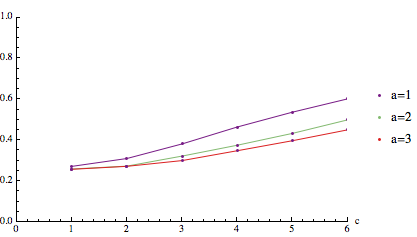
\includegraphics[width=0.8\textwidth]{images/real_sampling.png}
\caption{Sampling algorithm for real merchants}\label{fig:real_sampling}
\end{minipage}
\hspace{0cm}
\begin{minipage}[h]{0.48\textwidth}
\centering
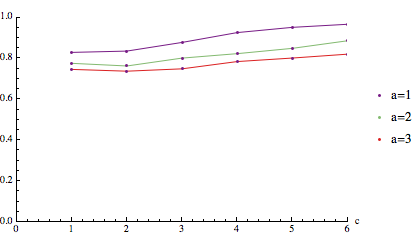
\includegraphics[width=0.8\textwidth]{images/real_greedy.png}
\caption{Greedy algorithm for real merchants}\label{fig:real_greedy}
\end{minipage}
\hspace{0cm}
\centering
\begin{minipage}[h]{0.48\textwidth}
\centering
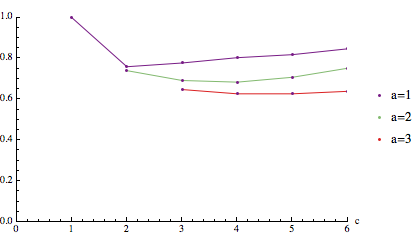
\includegraphics[width=0.8\textwidth]{images/real_partition.png}
\caption{Partition algorithm for real merchants}\label{fig:real_partition}
\end{minipage}
\vspace{-0.2in}
\end{figure} \vs

From these results, we can see that that greedy performs exceptionally well when $c$ gets even moderately large.
For the realistic value of $c=6$, the greedy algorithm produced a solution that was 85\% optimal for all the
merchants we tested. For several of the merchants, it in fact performed almost optimally starting from $a=2$. \vs

The partition is also promising, especially when the $a$ value we're aiming for is low. Indeed, when $a=1$ or $a=2$,
it's on average comparable to greedy though not nearly as good as the simulated runs would suggest. In fact, in some
instances partition can beat the performance of the greedy algorithm. However, as $a$ gets larger, the partition
algorithm gets worse faster than the other algorithms since the matchings it finds are not informed of the other
matchings. \vs

The sampling algorithm does mostly fine in real life data, but only when $c$ get rather large. It's obviously worse
than greedy, but unlike the partition algorithm its performance improves dramatically as $c$ gets larger, and its 
performance doesn't get worse as quickly when $a$ gets larger. Therefore, as $c$ gets larger, it becomes a viable
alternative to greedy especially in cases where we can't even pay the $O(|L|+|R|)$ memory cost of the greedy algorithm.
It is therefore impractical to use on all but the largest of data sets.